% !TEX encoding = UTF-8
% !TEX TS-program = pdflatex
% !TEX root = ../tesi.tex
% !TEX spellcheck = it-IT

%**************************************************************
\chapter{Introduzione}
\label{cap:introduzione}
%**************************************************************
xxxx
Introduzione al contesto applicativo.\\

\noindent Esempio di utilizzo di un termine nel glossario \\
\gls{api}. \\

\noindent Esempio di citazione in linea \\
\cite{site:agile-manifesto}. \\

\noindent Esempio di citazione nel pie' di pagina \\
citazione\footcite{womak:lean-thinking} \\

%**************************************************************
\section{L'azienda}

VIC è stata fondata da Alessio Bisutti che, dopo aver sviluppato una lunga esperienza nel campo ispettivo, ha deciso di costituire una società in grado di offrire ai propri clienti un servizio professionale, chiaro ed affidabile, appoggiandosi sulle nuove tecnologie.\\
VIC iniziò a Venezia 7 anni fa come piccola società di ispezione locale ed ora il gruppo VIC è uno dei più grandi attori del mercato globale.\\
Fin dall'inizio, l'obiettivo principale di VIC è stata la riduzione del tempo tra ispezione e reporting al cliente. Ora l'obiettivo è raggiunto, perché VIC sta fornendo ai suoi clienti tutti i risultati e le informazioni importanti in tempo reale, senza alcun ritardo, grazie agli investimenti fatti nel campo della tecnologia e delle applicazioni mobile.\\
VIC è la prima ed unica azienda in campo ispettivo ad offrire un'ampia gamma di servizi tecnologici a completa disposizione dei propri clienti. 

%**************************************************************
\section{L'idea}

Mansioni come determinare la corretta forma, peso, quantità e dimensioni degli oggetti da ispezionare sono tra le più importanti per i controlli effettuati dall'azienda.\\
Gli ispettori possono scattare molte fotografie, prendere appunti e sfruttare la loro esperienza per fornire stime accurate; si è manifestata però la necessità di affiancare queste ultime a dei dati quanto più possibile oggettivi e rapidi da ottenere.\\
Da qui nasce l'idea di fornire agli ispettori uno strumento informatico in grado di effettuare queste stime. Grazie alla ricostruzione computerizzata resa disponibile dai \emph{Tango device} sarà possibile non solo visualizzare su uno schermo il modello 3D del soggetto della ispezione, ma anche ottenere ulteriori vantaggi quali:
\begin{itemize}
	\item Avere una stima del volume e quindi del peso della materia prima.
	\item Confrontare l'oggetto con un modello idea, permettendo così un rapido controllo eventuali di danni o deformazioni.
\end{itemize}

\section{Il Prodotto}
L'applicazione prodotta risponde, in maniera minimale, alle esigenze citate nel punto precedente.\\
La sua realizzazione presenta molti punti critici e rischi piuttosto difficili da prevedere. Per questo sono stati realizzati molti prototipi, al fine di escludere vie non percorribili e trovare una soluzione soddisfacente.\\
Lo scopo principale della applicazione lato tablet è quello di rilevare ed elaborare un corretto \emph{Point Cloud} dell'oggetto che si vuole ispezionare.\\
Un \emph{Point Cloud} non è altro che una descrizione algebrica di un oggetto tridimensionale ottenuta tramite un insieme, il più possibile fitto, di punti che lo compongono. I dispositivi Tango infatti, grazie al sensore di profondità, cercano di rilevare le triplette di coordinate del maggior numero di punti possibile. Sfruttando questi dati è possibile posizionare dei punti nello spazio in maniera da fornire all'utente una rappresentazione comprensibile dell'oggetto.
\begin{figure}[!h] 
    \centering 
    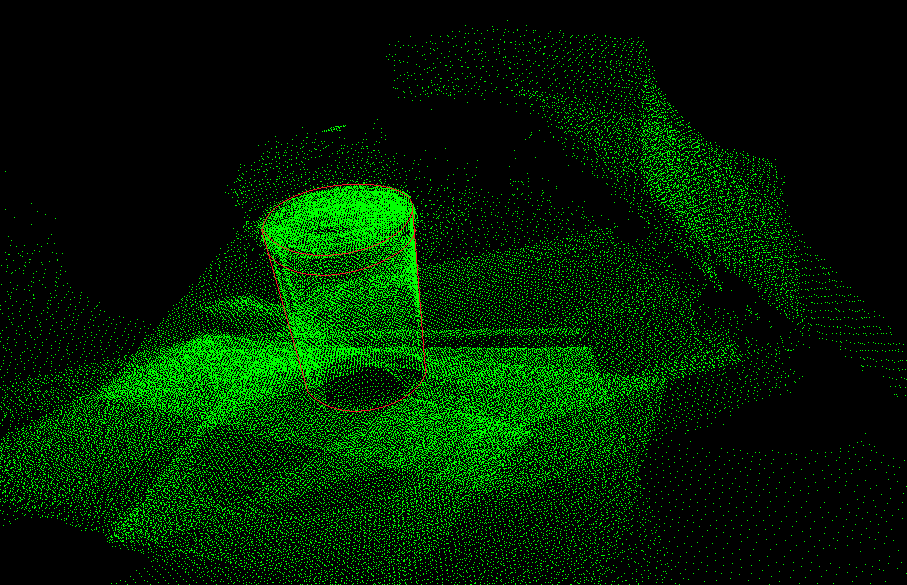
\includegraphics[width=1.0\columnwidth]{pointClouds/bidoneConico.png} 
    \caption{Point Cloud di un bidone Conico}
\end{figure}


\subsection{Primo prototipo}
Il primo protitpo realizzato risponde all'esigenza di catturare e salvare in formato leggibile da un \emph{render} grafico i dati forniti dal sensore di profondità.
Nella sua semplicità ha dato modo allo studente di testare la stabilità delle \emph{API} e produrre della documentazione interna che riportava quali fossero i metodi delle \emph{API} da utlizzare e quali fossero invece quelli poco stabili, sperimentali o addirittura non ancora implementati dal produttore.

\subsection{Secondo prototipo: Cloude}
\subsubsection{Affrontare la discrepanza tra coordinate assolute e coordinate relative}
Un solo \emph{Point Cloud} non è sufficiente a ricostruire un oggetto. Ovviamente il dispositivo, registrando la nuvola di punti inquadrata in un determinato istante, riesce a rilevare solamente i punti che "riesce a vedere": i punti presenti nella parte posteriore dell'oggetto scansionato non possono essere "visti" e conseguentemente nemmeno misurati. Se si vuole avere una ricostruzione completa e non solamente di una facciata è necessario prendere più rilevazioni ed integrarle.\\
Le seuguenti immagini mostrano il \emph{Point Cloud} che descrive la parte anteriore di una scatola rettangolare; dato che la ripresa è stata effettuata da di fronte ed in alto solo le facce superiore ed anteriore sono state memorizzate, mentre delle altre non si hanno dati. I contorni sono stati evidenziati successivamente per permettere una migliore comprensione della forma.
\begin{figure}[!h] 
    \centering 
    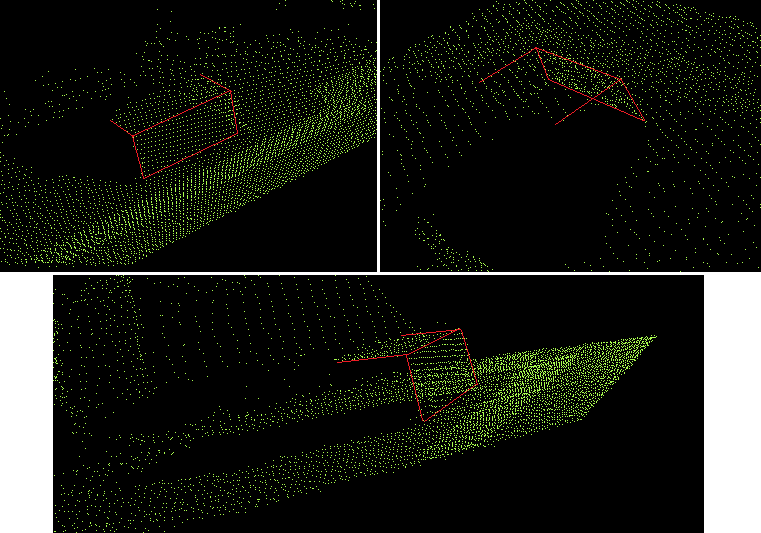
\includegraphics[width=1.0\columnwidth]{pointClouds/singoloShot.png} 
    \caption{Un singolo \emph{Point Cloud}}
\end{figure}
\subsubsection{Approccio}
Questo prototipo, denominato \emph{Cloude}, è stato realizzato allo scopo di rispondere a questa esigenza. L'idea che ne sta a fondamento è la seguente:
\begin{itemize}
	\item Permettere all'utente di scattare alcune foto all'oggetto, quindi di rilevare diversi \emph{Point Cloud}.
	\item Tenere costamente traccia della posizione del dispositivo, in particolare delle posizioni nei momenti in cui vengono scattate le foto.
	\item Usare la posizione relativa al \emph{Point Cloud} per translare e ruotare lo stesso punto a punto, riducendo così le coordinate a dei valori assoluti.
	\item Ora le nuvole di punti registrate sono sovrapponibili le une con le altre e forniscono una prima ricostruzione dell'oggetto.
\end{itemize}

\subsection{Terzo protipo: Samba}
Il prototipo precedente generava delle ricostruzioni riconoscibili, ma piuttosto imprecise.\\
Una analisi dello stesso ha fatto emergere diverse criticità che sono state documentate, assieme alle possibili soluzioni, all'interno di un documento descrittivo. Quest'ultimo è stato alla base dello svilluppo di \emph{Samba}.
\subsubsection{Eccessiva complessità dell'elaborazione}
\emph{Cloude} sfrutta un metedo delle librerie \emph{Tango} che transforma le coordinate di un singolo punto in coordinate assolute fruttando la posizione relativa a cui si trovava il dispositivo, permette di scrivere poco codice, ma ha una elevata complessità. Ciò comporta un sensibile rallentamento dell'elaborazione dei \emph{Point Cloud}. Un \emph{cloud} medio conta intorno ai 90000 punti e con questo approccio richiede mediamente 1,5-2 secondi per essere completamente elaborato, tempo non accettabile per lo scopo per cui l'applicazione è pensata.\\
In \emph{Samba} è stato cambiato radicalmente approccio:
\begin{itemize}
	\item Ad ogni \emph{Point Cloud} viene associata una matrice di transformazione e non la posizione stessa.
	\item In questo modo è sufficiente moltiplicare ogni punto (vettore) per la matrice, che viene calcolata una sola volta per ogni \emph{Poit Cloud}. 
	\item Si è ottenuta così una complessità di \texttt{O(n)} sul numero dei punti da transformare riducendo i tempi di elaborazione da 1,5-2s a circa 200ms (sullo stesso dispositivo).
\end{itemize}
\subsubsection{Bassa qualità delle ricostruzioni}
Nelle ricostruzioni generate da \emph{Cloude} gli oggetti appaiono deformati, spesso i vari \emph{Point Cloud} non si sovrappongono correttamente generando fenomeni di \emph{ghosting}, talvolta rendendo addirittura irriconoscibile l'oggetto.\\
Questo è dovuto ad una scorretta stima della posizione del dispositivo, che induce il calcolo di una erronea matrice di transformazione, e quindi ad un errato posizionamento delle nuvole di punti all'interno dello spazio.\\
Il fenomeno in questione è detto \emph{"drifting"}: i \emph{device Tango}, esattamente come le più comuni applicazioni in realtà aumentata, utilizzano la tecnica del \emph{Motion Tracking} che consiste nel calcolare la propria posizione frequentemente ed in maniera relativa alla coordinate acquisite nella stima precedente. Per quando queste stime siano estremamente precise generano una catena di piccoli errori che sommati tra loro molto presto portano ad una importante discrepanza tra la posizione stimata dal dispositivo e quella reale. Ad esempio partendo da una determinata posizione e camminando in cerchio è praticamente impossibile che la traiettoria stimata passi nuovamente per il punto di partenza.
\begin{figure}[!h] 
    \centering 
    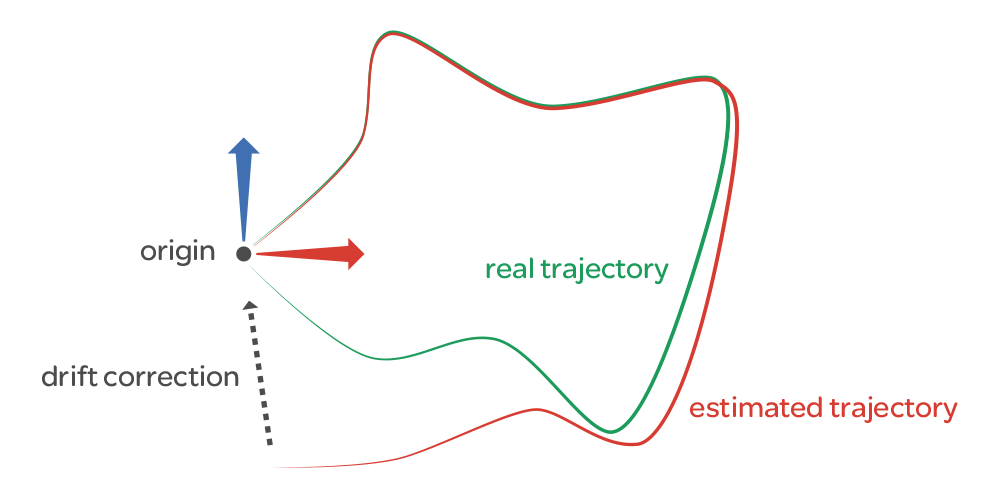
\includegraphics[width=0.9\columnwidth]{varie/Drift_Correction.png} 
    \caption{Motion Tracking}
\end{figure}
Ciò è un limite fisico dei dispositivi, ed è nella pratica impossibile da eliminare, in quanto sarebbe necessario azzerare completamente gli errori relativi.\\
La tecnologua \emph{Tango} però fonrnisce un altro meccanismo di localizzazione: l'\emph{Area Learning}. Le applicazioni ideate per questo tipo di dispositivi infatti hanno la possibilità di mantenere memoria degli spazi che visitano, e successivamente usare queste informazioni per localizzarsi.\\
Il meccanismo è piuttosto simile a quello della memoria spaziale umana: una persona portata bendata all'interno di un edificio sconosciuto, una volta liberata, non avrà alcun mezzo per intuire dove si trovi; se invece la stessa persona fosse condotta all'interno della propria abitazione, alla prima sbirciata noterebbe immediatamente qualche particolare che gli farebbe immediatamente recuperare l'orientamento.\\
Allo stesso modo il tablet è in grado memorizzare alcune \emph{features} all'interno dell'ambiente ed usarle come faro per la triangolazione. \\
Memorizzare completamente un ambiente tuttavia è una operazione che richiede parecchio tempo e costringe l'utente a muoversi per diversi minuti inquadrando tutti i dettagli del luogo dove si trova. Per rendere l'aplicazione maggiornamente responsiva e più vicina alle esigenze dell'utenza \emph{Samba} adotta un approccio detto \emph{Drift Correction}: inzialmente è richiesto all'utente di inquadrare per una ventina di secondi l'ambiente, in maniera da permettere la creazione di una minimale memorizzazione, successivamente il \emph{Motion Tracking} è usato per piccoli spostamenti ma viene corretto nonappena venga inquadrata qualcuna delle (poche) \emph{features} memorizzate. Trasparentemente all'utente, in background, il processo di \emph{Area Learning} continua, memorizzando sempre nuovi dettagli e conseguentemente aumentando sempre più la qualità della registazione.\\

\subsection{Dimensioni eccessive dei file, ridondanza dei punti sovrapposti}
Data la grande mole di punti registrati dai sensori di profondità i \emph{file} contenenti le ricostruzioni generati da \emph{Cloude} sono di dimensione eccessiva, anche più di 10Mb una decina scatti.
Considerando che idealmente gli scatti da riprendere potrebbero essere molti e spesso dovranno essere inviati al \emph{Server} tramite connessione a consumo il peso di questi \emph{file} non è da trascurare.\\
Inoltre c'è una grossa ridondanza di punti: è comune caso d'uso che una stessa zona venga inquadrata in più scatti, quindi tali \emph{Point Cloud} ruotati ed uniti presenterebbero molti punti con le stesse coordinate e semplicemente sovrapposti, qunidi sera dare alcuna informazione aggiuntiva.\\
\emph{Samba} risolve questo problema utilizzando un leggero \emph{voxeling}, ovvero suddividendo lo spazio in cubi o \emph{voxel} di lato prefissato e registrando quali sono i \emph{voxel} che contengono i punti della nuvola.





%**************************************************************
\section{Organizzazione del testo}
xxxx
\begin{description}

    \item[{\hyperref[cap:processi-metodologie]{Il secondo capitolo}}] descrive ...
    
    \item[{\hyperref[cap:descrizione-stage]{Il terzo capitolo}}] approfondisce ...
    
    \item[{\hyperref[cap:analisi-requisiti]{Il quarto capitolo}}] approfondisce ...
    
    \item[{\hyperref[cap:progettazione-codifica]{Il quinto capitolo}}] approfondisce ...
    
    \item[{\hyperref[cap:verifica-validazione]{Il sesto capitolo}}] approfondisce ...
    
    \item[{\hyperref[cap:conclusioni]{Nel settimo capitolo}}] descrive ...
\end{description}

Riguardo la stesura del testo, relativamente al documento sono state adottate le seguenti convenzioni tipografiche:
\begin{itemize}
	\item gli acronimi, le abbreviazioni e i termini ambigui o di uso non comune menzionati vengono definiti nel glossario, situato alla fine del presente documento;
	\item per la prima occorrenza dei termini riportati nel glossario viene utilizzata la seguente nomenclatura: \emph{parola}\glsfirstoccur;
	\item i termini in lingua straniera o facenti parti del gergo tecnico sono evidenziati con il carattere \emph{corsivo}.
\end{itemize}